% Q11: flat subdivision of the equilateral triangle before folding.
% Coordinates enforce the stated midpoints; they do not encode a perspective after folding.
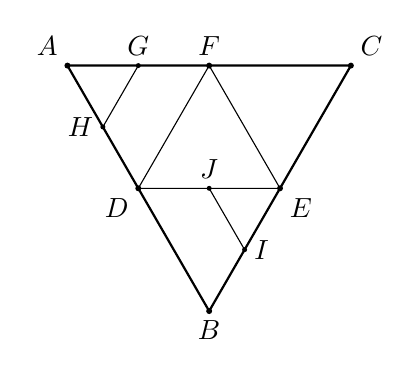
\begin{tikzpicture}[scale=0.9,line cap=round,line join=round]
  \coordinate (A) at (0,3.4641);
  \coordinate (C) at (4,3.4641);
  \coordinate (B) at (2,0);
  \coordinate (D) at (1,1.73205);
  \coordinate (E) at (3,1.73205);
  \coordinate (F) at (2,3.4641);
  \coordinate (G) at (1,3.4641);
  \coordinate (H) at (0.5,2.59808);
  \coordinate (I) at (2.5,0.86603);
  \coordinate (J) at (2,1.73205);

  \draw[thick] (A)--(C)--(B)--cycle;
  \draw (D)--(E)--(F)--cycle;
  \draw (G)--(H) (J)--(I);

  \fill (A) circle (1.2pt) node[above left] {$A$};
  \fill (B) circle (1.2pt) node[below] {$B$};
  \fill (C) circle (1.2pt) node[above right] {$C$};
  \fill (D) circle (1.2pt) node[below left] {$D$};
  \fill (E) circle (1.2pt) node[below right] {$E$};
  \fill (F) circle (1.2pt) node[above] {$F$};
  \fill (G) circle (1pt) node[above] {$G$};
  \fill (H) circle (1pt) node[left] {$H$};
  \fill (I) circle (1pt) node[right] {$I$};
  \fill (J) circle (1pt) node[above] {$J$};
\end{tikzpicture}
